\documentclass[11pt]{article}

\usepackage{amsmath}
\usepackage{amssymb}
\usepackage{mathtools}
\usepackage[margin=1in]{geometry}
\usepackage{booktabs}
\usepackage{longtable}
\usepackage{tikz}
\usetikzlibrary{arrows.meta,positioning,calc,shapes.geometric}
\usepackage[numbers,sort&compress]{natbib}
\usepackage{hyperref}
\usepackage[capitalise,noabbrev]{cleveref}

\hypersetup{colorlinks=true,linkcolor=blue!50!black,citecolor=blue!50!black,urlcolor=blue!50!black}

% ---- math operators / shortcuts ----
\DeclareMathOperator{\tr}{tr}
\DeclareMathOperator*{\argmin}{arg\,min}
\DeclareMathOperator{\diag}{diag}
\DeclareMathOperator{\clip}{clip}
\newcommand{\R}{\mathbb{R}}
\newcommand{\W}{\mathbb{W}}
\newcommand{\Xset}{\mathbb{X}}
\newcommand{\Uset}{\mathbb{U}}
\newcommand{\norm}[1]{\left\lVert #1 \right\rVert}
\newcommand{\bx}{\bar{x}}
\newcommand{\bu}{\bar{u}}
\newcommand{\bp}{\bar{p}}
\newcommand{\code}[1]{\texttt{#1}}
\newcommand{\fov}{\mathrm{fov}}
\newcommand{\opt}{\mathrm{opt}}

\title{\textbf{A Mathematical Derivation of an Observability-Coupled\\
Aerial--Ground Cooperative Tracking System:\\ Event-Triggered Tube MPC and Belief-Space Guidance}}
\author{Theoretical companion to the \code{ugv\_uav\_control} package}
\date{\today}

\begin{document}
\maketitle

\begin{abstract}
This document is the standalone theoretical companion to the code report (\code{report.html}) for the
\code{ugv\_uav\_control} ROS\,2 package. It derives, from textbook foundations, the mathematics of a
cooperative system in which a single downward-facing camera on a quadrotor (UAV) is the only sensor for a
ground vehicle (UGV). The work extends \citet{ferreira2024aerial} in two ways: (i) the UAV trajectory is
planned online by event-triggered Tube Model Predictive Control (MPC) rather than tracking fixed waypoints,
and (ii) the Extended Kalman Filter (EKF) covariance is injected into both controllers' cost functions,
creating a bidirectional perception--control loop. Throughout, we separate the \emph{idealized} theory
(constrained robust MPC with a minimal robust positively invariant set) from what the implementation
\emph{actually} computes (an ellipsoidal tube with loaded/fallback gains, a single-integrator UAV model,
and a view-quality-scaled measurement noise). Deviations are catalogued in \cref{sec:impl}. We state the
stability and recursive-feasibility results we rely on and are explicit about which guarantees are proven,
which are inherited from cited theorems under assumptions, and which are only empirically supported.
\end{abstract}

\tableofcontents

% =====================================================================
\section{Notation and symbol table}
\label{sec:notation}

All symbols are defined once here and again at first use. ``dim'' gives the object type;
$n$ denotes a scalar, $\R^n$ a vector, $\R^{n\times m}$ a matrix. Time index $k$ is discrete.

{\small
\begin{longtable}{@{}l l l l@{}}
\toprule
Symbol & Meaning & Dim / units & First used \\
\midrule
\endfirsthead
\toprule
Symbol & Meaning & Dim / units & First used \\
\midrule
\endhead
\multicolumn{4}{c}{\emph{UGV state and model}} \\
$x_{\text{ugv}}=[x,y,\theta,v,\omega]^\top$ & UGV state (pose + body velocities) & $\R^5$; m, rad, m/s, rad/s & \cref{sec:models} \\
$u_{\text{ugv}}=[v_{\text{cmd}},\omega_{\text{cmd}}]^\top$ & UGV velocity command & $\R^2$; m/s, rad/s & \cref{sec:models} \\
$\alpha_v,\alpha_\omega$ & actuator-lag rates ($1/\tau$) & $2.0,\,5.0$ s$^{-1}$ & \cref{sec:models} \\
$\bar v,\bar\omega$ & trapezoidal mean velocities & m/s, rad/s & \cref{sec:models} \\
$F_k=\partial f/\partial x$ & UGV process Jacobian & $\R^{5\times5}$ & \cref{sec:ekf} \\
$Q$ & UGV process-noise covariance & $\R^{5\times5}$ & \cref{sec:ekf} \\
\midrule
\multicolumn{4}{c}{\emph{UAV state and model}} \\
$p=[p_x,p_y,p_z]^\top$ & UAV position & $\R^3$; m & \cref{sec:models} \\
$u=[v_x,v_y,v_z]^\top$ & UAV velocity command (control) & $\R^3$; m/s & \cref{sec:models} \\
$A_d,B_d$ & discrete UAV dynamics matrices & $I_3,\ \Delta t\,I_3$ & \cref{sec:models} \\
$\bp_k,\bu_k$ & nominal UAV state / input & $\R^3$ & \cref{sec:tube} \\
$e_k=p_k-\bp_k$ & UAV tracking error & $\R^3$; m & \cref{sec:tube} \\
$K$ & ancillary feedback gain & $\R^{3\times3}$ & \cref{sec:tube} \\
$P_0$ & tube ellipsoid shape matrix & $\R^{3\times3}$, $\succ0$ & \cref{sec:tube} \\
$\alpha_k$ & adaptive tube radius & scalar & \cref{sec:tube} \\
$w_k$ & additive disturbance & $\R^3$, $w_k\in\W$ & \cref{sec:refs} \\
$\W,\Omega$ & disturbance set, (m)RPI set & compact $\subset\R^3$ & \cref{sec:refs},\,\cref{sec:tube} \\
$g$ & UGV predicted goal for UAV planner & $\R^3$; m & \cref{sec:tube} \\
\midrule
\multicolumn{4}{c}{\emph{Estimation and perception}} \\
$\mu,\Sigma$ & EKF mean, covariance & $\R^5,\ \R^{5\times5}$ & \cref{sec:ekf} \\
$H$ & measurement matrix & $\R^{m\times5}$ & \cref{sec:ekf} \\
$R_k,R_{\text{full}},R_{\text{odom}}$ & measurement-noise covariances & matrices & \cref{sec:ekf} \\
$q_k\in(0,1]$ & view-quality score & scalar & \cref{sec:viewquality} \\
$d$ & horizontal UAV$\to$UGV distance & m & \cref{sec:viewquality} \\
$r_{\fov}=z\tan(\fov/2)$ & ground FoV radius & m & \cref{sec:constraints} \\
$\fov$ & camera full field-of-view angle & $1.047$ rad ($60^\circ$) & \cref{sec:constraints} \\
$z_\opt,\sigma_z$ & precision-optimal altitude, its spread & $5$ m, $3$ m & \cref{sec:viewquality} \\
$\sigma_{xy}=r_{\fov}/2$ & centering spread & m & \cref{sec:viewquality} \\
$\beta$ & sigmoid sharpness (FoV roll-off) & $5$ & \cref{sec:viewquality} \\
\midrule
\multicolumn{4}{c}{\emph{Cost weights and horizons}} \\
$N$ & prediction horizon (UAV $10$, UGV $5$) & steps & \cref{sec:mpc} \\
$\Delta t$ & time step ($0.2$ s MPC, $0.05$ s EKF) & s & \cref{sec:mpc} \\
$w_\ell=\mathrm{linspace}(1,2,N)$ & UAV horizon weight vector & $\R^N$ & \cref{sec:tube} \\
$w_z,w_{\text{alt}}$ & UAV altitude / visibility weights & $3,\,50$ & \cref{sec:tube} \\
$w_d,w_h,w_r,\lambda,w_{\fov}$ & UGV cost weights & $10,10,5,1,2$ & \cref{sec:beliefmpc} \\
$c_{\fov}(\cdot)$ & FoV-exit penalty (hinge$^2$) & scalar & \cref{sec:beliefmpc} \\
\bottomrule
\end{longtable}
}

\noindent\textbf{Convention.} Bars ($\bp,\bu$) denote nominal (planned) quantities; hats are not used.
$\norm{\cdot}$ is the Euclidean norm; $\norm{e}_{P_0}^2 := e^\top P_0 e$. $\ominus$ is the Pontryagin
(Minkowski) set difference. A matrix is \emph{Schur} if all eigenvalues lie strictly inside the unit disc.

% =====================================================================
\section{System representations}
\label{sec:models}

\begin{figure}[t]
\centering
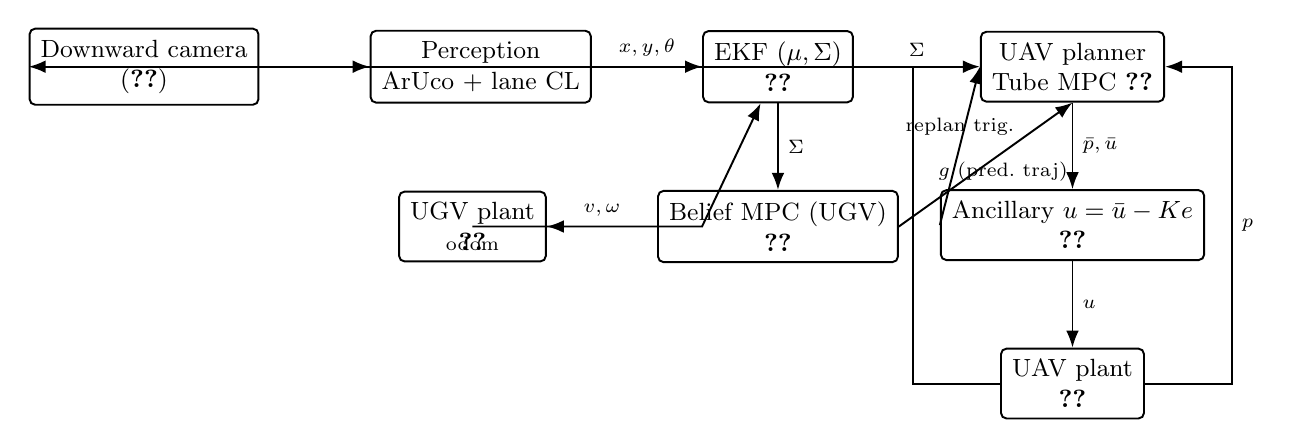
\begin{tikzpicture}[
  >=Latex, line width=0.7pt, font=\small,
  block/.style={draw, rounded corners=2pt, align=center, inner sep=4pt, minimum height=8mm},
  sig/.style={->, line width=0.7pt}]
\node[block] (cam) {Downward camera\\(\cref{sec:constraints})};
\node[block, right=14mm of cam] (perc) {Perception\\ArUco + lane CL};
\node[block, right=14mm of perc] (ekf) {EKF $(\mu,\Sigma)$\\\cref{sec:ekf}};
\node[block, below=11mm of ekf] (bmpc) {Belief MPC (UGV)\\\cref{sec:beliefmpc}};
\node[block, left=14mm of bmpc] (ugv) {UGV plant\\\cref{eq:ugv_disc}};
\node[block, right=16mm of ekf] (plan) {UAV planner\\Tube MPC \cref{sec:tube}};
\node[block, below=11mm of plan] (anc) {Ancillary $u=\bu-Ke$\\\cref{sec:eventtrigger}};
\node[block, below=11mm of anc] (uav) {UAV plant\\\cref{eq:uav_disc}};

\draw[sig] (cam) -- (perc);
\draw[sig] (perc) -- node[above,font=\scriptsize]{$x,y,\theta$} (ekf);
\draw[sig] (ekf) -- node[right,font=\scriptsize]{$\Sigma$} (bmpc);
\draw[sig] (bmpc) -- node[above,font=\scriptsize]{$v,\omega$} (ugv);
\draw[sig] (ugv) |- node[below,font=\scriptsize,pos=0.25]{odom} (ekf.west|-ugv) -- (ekf);
\draw[sig] (ekf) -- node[above,font=\scriptsize]{$\Sigma$} (plan);
\draw[sig] (bmpc.east) -- node[below,font=\scriptsize,pos=0.6]{$g$ (pred.\ traj)} (plan.south);
\draw[sig] (plan) -- node[right,font=\scriptsize]{$\bp,\bu$} (anc);
\draw[sig] (anc) -- node[right,font=\scriptsize]{$u$} (uav);
\draw[sig] (anc.west) -- node[above,font=\scriptsize]{replan trig.} (plan.west);
\draw[sig] (uav.east) -- ++(1.1,0) |- node[right,font=\scriptsize,pos=0.25]{$p$} (plan.east);
\draw[sig] (uav.west) -- ++(-1.1,0) |- (cam.west);
\end{tikzpicture}
\caption{Controller architecture and the two coupling paths. The camera is the only sensor; perception feeds
the EKF, whose covariance $\Sigma$ enters \emph{both} the belief MPC (UGV) and the UAV Tube-MPC planner. The
belief MPC's predicted trajectory is the goal $g$ for the UAV planner; the ancillary loop tracks the nominal
plan and requests replans on events. Arrows back to the camera close the perception loop.}
\label{fig:arch}
\end{figure}

\subsection{UGV model}
\citet{ferreira2024aerial} model the ground vehicle as a front-steered bicycle. Writing the rear-axle
position $(x,y)$, heading $\theta$, longitudinal speed $v$, and steering angle $\delta$ with wheelbase $L$,
the kinematic bicycle model (their Eq.~6) is
\begin{equation}
\dot x = v\cos\theta,\qquad \dot y = v\sin\theta,\qquad \dot\theta = \frac{v}{L}\tan\delta .
\label{eq:bicycle}
\end{equation}
Under the no-slip and small-steering assumptions used by ECC (lateral forces negligible, $\tan\delta\approx
L\omega/v$ for commanded yaw rate $\omega$), \cref{eq:bicycle} reduces to the unicycle (their Eq.~7)
\begin{equation}
\dot x = v\cos\theta,\qquad \dot y = v\sin\theta,\qquad \dot\theta = \omega .
\label{eq:unicycle}
\end{equation}
The TurtleBot3 is differential-drive, so \cref{eq:unicycle} is exact for it (no wheelbase appears).

\paragraph{Discrete-time form actually implemented.}
The code (\code{ugv\_model.py}) augments \cref{eq:unicycle} with \emph{first-order actuator lag}: the
commanded velocities are not reached instantaneously, so $v$ and $\omega$ become states. With step
$\Delta t$, lag rates $\alpha_v=2$ ($\tau_v=0.5$\,s) and $\alpha_\omega=5$ ($\tau_\omega=0.2$\,s),
\begin{align}
v_{k+1} &= v_k + \alpha_v\,(v_{\text{cmd}}-v_k)\,\Delta t, &
\omega_{k+1} &= \omega_k + \alpha_\omega\,(\omega_{\text{cmd}}-\omega_k)\,\Delta t .
\label{eq:lag}
\end{align}
Pose is then integrated with the \emph{trapezoidal mean} velocities
$\bar v=\tfrac12(v_k+v_{k+1})$, $\bar\omega=\tfrac12(\omega_k+\omega_{k+1})$, using the exact
constant-curvature arc solution
\begin{equation}
\boxed{\;
\begin{aligned}
x_{k+1} &= x_k + \frac{\bar v}{\bar\omega}\bigl(\sin(\theta_k+\bar\omega\,\Delta t)-\sin\theta_k\bigr),\\
y_{k+1} &= y_k - \frac{\bar v}{\bar\omega}\bigl(\cos(\theta_k+\bar\omega\,\Delta t)-\cos\theta_k\bigr),\\
\theta_{k+1} &= \theta_k + \bar\omega\,\Delta t,
\end{aligned}\;}
\label{eq:ugv_disc}
\end{equation}
valid for $|\bar\omega|\ge10^{-4}$; otherwise the straight-line limit
$x_{k+1}=x_k+\bar v\cos\theta_k\,\Delta t$, $y_{k+1}=y_k+\bar v\sin\theta_k\,\Delta t$ is used.
\Cref{eq:ugv_disc} follows from integrating \cref{eq:unicycle} over $[k\Delta t,(k{+}1)\Delta t]$ at
constant $\bar v,\bar\omega$, and is exact for that segment (it avoids Euler drift). The full state is
\[
x_{\text{ugv}} = [x,\,y,\,\theta,\,v,\,\omega]^\top \in\R^5, \qquad
u_{\text{ugv}} = [v_{\text{cmd}},\,\omega_{\text{cmd}}]^\top \in\R^2 .
\]

\subsection{UAV model}
\label{sec:uavmodel}
\emph{The implementation does not use a double integrator.} Both the planner (\code{uav\_mpc\_node.py}) and
the ancillary tracker (\code{uav\_ancillary\_node.py}) treat the quadrotor as a \textbf{point-mass single
integrator} whose control input is the commanded \emph{velocity} (the Gazebo \code{VelocityControl} plugin
closes the underlying attitude/thrust loops). With position $p=[p_x,p_y,p_z]^\top$ and velocity command
$u=[v_x,v_y,v_z]^\top$,
\begin{equation}
\boxed{\,p_{k+1} = p_k + \Delta t\,u_k + w_k\,}
\qquad\Longrightarrow\qquad
A_d = I_3,\quad B_d = \Delta t\,I_3,
\label{eq:uav_disc}
\end{equation}
with $w_k\in\W$ the disturbance (\cref{sec:refs}). The planner enforces velocity bounds
$v_x,v_y\in[-1.5,1.5]$ m/s and $v_z\in[-1,1]$ m/s. Vertical velocity is a genuine decision variable, so
altitude is planned, not fixed --- the central modelling difference from ECC, where altitude is constant
and the UAV merely tracks pre-set waypoints.

\begin{quote}\small
\textbf{Remark (idealized vs.\ implemented).} A second-order $[p,v]^\top$ double-integrator with acceleration
input $a=[a_x,a_y,a_z]^\top$ and gravity compensation, $\dot p = v,\ \dot v = a - g e_3$, is the more faithful
rigid-body abstraction and is what a from-scratch Tube-MPC design would normally use. We retain the
single-integrator form \cref{eq:uav_disc} throughout because that is what the code optimizes and tracks; the
double-integrator alternative is noted only here and in \cref{sec:impl}.
\end{quote}

% =====================================================================
\section{Reference and disturbance models}
\label{sec:refs}

\paragraph{Reference trajectory.} The UAV nominal trajectory $\{\bp_k,\bu_k\}_{k=0}^{N}$ is \emph{not}
externally given (as in ECC); it is produced online by the planner of \cref{sec:tube}. The planner's
\emph{goal} $g\in\R^3$ is the UGV's predicted position at the end of the UGV's own horizon, read from the
\code{/ugv\_predicted\_traj} message published by the belief-space MPC (\cref{sec:beliefmpc}). Thus the
reference for the aerial loop is itself the output of the ground loop's predictive model --- one direction of
the perception--control coupling.

\paragraph{Disturbance set.} We model unmodelled velocity-tracking error, wind, and plugin latency as a
bounded additive disturbance $w_k\in\W$. For the robust-MPC theory of \cref{sec:tube,sec:validation} we make
the standard assumption \citep{mayne2005robust}:
\begin{description}
\item[\textnormal{(A1)}] $\W\subset\R^3$ is compact, convex, and contains the origin: $0\in\W$.
\end{description}
The code does not estimate $\W$ explicitly; the tube ellipsoid and its adaptive radius $\alpha_k$
(\cref{sec:tube}) act as a surrogate for the resulting invariant set. This is one of the deviations recorded
in \cref{sec:impl}.

% =====================================================================
\section{Constraints}
\label{sec:constraints}

\paragraph{State constraints $\Xset$.} The natural workspace constraints are altitude bounds
$z_{\min}\le p_z\le z_{\max}$ with $z_{\min}=3,\ z_{\max}=10$ m (declared in \code{uav\_mpc\_node.py}).
\emph{These are declared but never enforced as optimization constraints in the code} (\cref{sec:impl});
altitude is shaped only softly through the cost.

\paragraph{Input constraints $\Uset$.} UAV velocity box
$\Uset_{\text{uav}}=\{u: |v_x|\le1.5,\,|v_y|\le1.5,\,|v_z|\le1\}$ (planner) and an ancillary saturation
$u\in[-1,1]^3$. UGV input box $\Uset_{\text{ugv}}=\{(v,\omega): 0\le v\le0.22,\ |\omega|\le2\}$.

\paragraph{Field-of-view constraint.} The single perception requirement is that the UGV remain inside the
downward camera's footprint. For a camera at altitude $z$ looking straight down with full opening angle
$\fov$, the imaged ground region is a disc of radius
\begin{equation}
r_{\fov}(z) = z\tan\!\left(\frac{\fov}{2}\right),
\label{eq:rfov}
\end{equation}
derived from the pinhole geometry: the extreme ray makes half-angle $\fov/2$ with the optical (vertical)
axis, so it meets the ground plane at horizontal offset $z\tan(\fov/2)$. With $p^{xy}=[p_x,p_y]^\top$ the UAV
ground projection and $p_{\text{ugv}}\in\R^2$ the UGV position, the geometric visibility condition is
\begin{equation}
\boxed{\;d := \norm{p^{xy}-p_{\text{ugv}}} \;\le\; r_{\fov}(z)\;}
\label{eq:fovconstraint}
\end{equation}
i.e.\ the target lies within the ground footprint. The code treats \cref{eq:fovconstraint} as a \emph{soft}
constraint everywhere (a penalty in the cost, \cref{sec:beliefmpc,sec:tube}), never as a hard constraint;
\cref{eq:rfov} uses the single full angle $\fov=1.047$, implicitly approximating the $640\times480$
(non-square) frame's footprint by a circle.

\paragraph{Other implicit constraints.} A blocking sanity-check parameter can suppress ArUco measurements over
a time window (dropout-robustness test); the perception pixel$\to$metre scale is computed once assuming
$z=5$ m (\cref{sec:viewquality}, \cref{sec:impl}).

% =====================================================================
\section{Standard MPC formulation}
\label{sec:mpc}

We recall nominal MPC \citep{mayne2000constrained,rawlings2017model} as the object we build on. Given the
discrete model $x_{k+1}=f(x_k,u_k)$, stage cost $\ell(\cdot)$, terminal cost $V_f$, and constraint sets
$\Xset,\Uset$, the finite-horizon optimal control problem solved at state $x$ is
\begin{equation}
\begin{aligned}
\min_{\mathbf{u}=\{u_0,\dots,u_{N-1}\}}\;
& \sum_{k=0}^{N-1}\ell(x_k,u_k) + V_f(x_N)\\
\text{s.t.}\quad & x_0 = x,\quad x_{k+1}=f(x_k,u_k),\\
& x_k\in\Xset,\ u_k\in\Uset,\ x_N\in\Xset_f .
\end{aligned}
\label{eq:nominalmpc}
\end{equation}
In receding-horizon implementation one applies only the first input $u_0^\star(x)$, advances the plant, and
re-solves at the next state. With a control-invariant terminal set $\Xset_f$ and terminal cost that is a local
Lyapunov function, \cref{eq:nominalmpc} is recursively feasible and the origin is asymptotically stable
\citep[Thm.~2.19]{rawlings2017model}. The remaining sections specialise this template: \cref{sec:tube} makes
it \emph{robust} to $w_k$, and \cref{sec:beliefmpc} augments the stage cost with estimation uncertainty.

% =====================================================================
\section{Tube MPC --- derivation from basics}
\label{sec:tube}

Tube MPC \citep{mayne2005robust} separates the controller into (i) a \emph{nominal} plan computed by MPC on
the disturbance-free system, and (ii) an \emph{ancillary} feedback law that keeps the true state inside a
``tube'' around the nominal plan despite $w_k$. We derive both for the single-integrator UAV
\cref{eq:uav_disc}.

\subsection{Nominal system and error dynamics}
The nominal (disturbance-free) system is
\begin{equation}
\bp_{k+1} = A_d\,\bp_k + B_d\,\bu_k = \bp_k + \Delta t\,\bu_k .
\label{eq:nominaldyn}
\end{equation}
Define the tracking error $e_k := p_k-\bp_k$. The ancillary law adds proportional feedback on the error:
\begin{equation}
\boxed{\,u_k = \bu_k - K\,e_k\,}
\label{eq:ancillary}
\end{equation}
(\code{uav\_ancillary\_node.py}; the command is then saturated to $[-1,1]^3$). Subtracting
\cref{eq:nominaldyn} from the true dynamics \cref{eq:uav_disc} and substituting \cref{eq:ancillary},
\begin{align}
e_{k+1}
&= (p_k+\Delta t\,u_k+w_k) - (\bp_k+\Delta t\,\bu_k) \notag\\
&= e_k + \Delta t\,(u_k-\bu_k) + w_k
 = e_k - \Delta t\,K e_k + w_k \notag\\
&= \underbrace{(I_3-\Delta t\,K)}_{=:A_K}\,e_k + w_k .
\label{eq:errordyn}
\end{align}
Robust regulation of the error requires $A_K=A_d-B_dK=I_3-\Delta t K$ to be \emph{Schur}. With the diagonal
gain actually used (fallback $K=2I_3$, $\Delta t=0.2$), $A_K=0.6\,I_3$, whose eigenvalues $0.6$ lie inside the
unit disc, so \cref{eq:errordyn} is exponentially stable in the nominal ($w=0$) case. Any loaded gain $K$
must satisfy the same Schur condition.

\subsection{Choice of $K$}
In the textbook design $K$ is the discrete-time LQR gain minimising
$\sum_k (e_k^\top Q_e e_k + u_k^\top R_e u_k)$, i.e.\ $K=(R_e+B_d^\top P B_d)^{-1}B_d^\top P A_d$ with $P$ the
solution of the discrete algebraic Riccati equation. \emph{This computation is not performed in the
repository.} The gain $K$ and the tube shape matrix $P_0$ are loaded from a precomputed file
(\code{tube\_params.npz}); when absent, the node falls back to $K=2I_3$ and $P_0=6.86\,I_3$. We therefore
treat $K,P_0$ as given design data satisfying the Schur and positive-definiteness requirements, and record in
\cref{sec:impl} that their principled (LQR/RPI) derivation belongs to an upstream stage absent from these
sources.

\subsection{Minimal robust positively invariant (mRPI) set}
For the error system \cref{eq:errordyn} with $A_K$ Schur and $w_k\in\W$ (A1), a set $\Omega\subset\R^3$ is
\emph{robust positively invariant (RPI)} if
\begin{equation}
A_K\,\Omega \oplus \W \subseteq \Omega ,
\label{eq:rpi}
\end{equation}
where $\oplus$ is the Minkowski sum. The \emph{minimal} RPI set is the limit
\begin{equation}
\Omega_\infty = \bigoplus_{i=0}^{\infty} A_K^{i}\,\W ,
\label{eq:mrpi}
\end{equation}
which converges because $A_K$ is Schur (the tail $\sum_{i\ge n}\norm{A_K^i}$ is geometrically summable)
\citep{rakovic2005invariant}. $\Omega_\infty$ is the smallest set such that $e_0\in\Omega_\infty\Rightarrow
e_k\in\Omega_\infty\ \forall k$ for every disturbance sequence; it is compact and contains the origin. In
practice one computes an outer $\varepsilon$-approximation $\Omega\supseteq\Omega_\infty$ by truncating
\cref{eq:mrpi} \citep{rakovic2005invariant}.

\paragraph{Ellipsoidal surrogate actually used.} Rather than computing \cref{eq:mrpi}, the code represents the
tube by the \emph{ellipsoid}
\begin{equation}
\boxed{\;\mathcal{E}(\alpha_k) = \{\,e\in\R^3 : e^\top P_0\,e \le \alpha_k^2\,\}\;}
\label{eq:ellipsoid}
\end{equation}
and declares the state ``inside the tube'' iff $e_k\in\mathcal{E}(\alpha_k)$. If $P_0$ is chosen as a Lyapunov
matrix for $A_K$ (i.e.\ $A_K^\top P_0 A_K - P_0\prec 0$) then a sublevel set $\{e^\top P_0 e\le c\}$ is
positively invariant for the nominal error dynamics, and for a suitable $c=\alpha^2$ accounting for $\W$ it is
RPI; \cref{eq:ellipsoid} is the implementation's stand-in for $\Omega$. Crucially the radius
\emph{adapts to estimation quality} (the extension over ECC):
\begin{equation}
\boxed{\;\alpha_k = \alpha_{\min} + (\alpha_{\max}-\alpha_{\min})\,
\clip\!\left(\frac{\tr\Sigma_{xy}-\tr_{\min}}{\tr_{\max}-\tr_{\min}},\,0,\,1\right)\;}
\label{eq:alpha}
\end{equation}
with $\alpha_{\min}=0.5,\ \alpha_{\max}=2,\ \tr_{\min}=0.005,\ \tr_{\max}=0.15$, and $\tr\Sigma_{xy}=
\Sigma_{xx}+\Sigma_{yy}$ the EKF horizontal position-covariance trace (\cref{sec:ekf}). The tube
\emph{breathes}: it tightens when the position estimate is sharp and loosens when perception degrades.

\subsection{Constraint tightening}
The nominal MPC must leave room for the error to occupy $\Omega$. Tube MPC tightens the original constraints by
the Pontryagin difference \citep{mayne2005robust}:
\begin{equation}
\bar\Xset = \Xset \ominus \Omega, \qquad \bar\Uset = \Uset \ominus K\Omega ,
\label{eq:tighten}
\end{equation}
where $\Xset\ominus\Omega=\{x: x\oplus\Omega\subseteq\Xset\}$. Planning the nominal trajectory inside
$\bar\Xset,\bar\Uset$ guarantees the true state/input stay in $\Xset,\Uset$ for any admissible disturbance,
since $x_k=\bp_k+e_k\in\bar\Xset\oplus\Omega\subseteq\Xset$. \emph{The code does not implement
\cref{eq:tighten}} (it has neither explicit $\Xset,\Uset$ nor $\Omega$); we state it because it is the formal
justification for why a correctly-sized tube yields constraint satisfaction, and its absence is a gap
(\cref{sec:impl}).

\subsection{The nominal planning problem (as implemented)}
The planner optimises the velocity sequence $\mathbf{u}=\{\bu_0,\dots,\bu_{N-1}\}\in\R^{N\times3}$, $N=10$,
$\Delta t=0.2$, over the single integrator. Predicted positions are
\begin{equation}
\bp_k = \bp_0 + \Delta t\sum_{j=0}^{k}\bu_j ,\qquad k=0,\dots,N-1,
\label{eq:cumsum}
\end{equation}
(the cumulative sum of \code{uav\_mpc\_node.py}; $\bp_k$ here is the position \emph{after} $k{+}1$ steps,
distinct from the base point $\bp_0$). With horizon weights
$w_\ell=\mathrm{linspace}(1,2,N)$ (later steps weighted more), $z_\opt$ the precision-optimal altitude,
$w_z=3$, $w_{\text{alt}}=50$, and goal $g$ (with $g^{xy}$ its horizontal part), the cost is
\begin{equation}
\boxed{\;
\begin{aligned}
J_{\text{uav}} =\; & \sum_{k} w_{\ell,k}\,\norm{\bp_k-g}^2
\;+\; w_z\sum_{k} w_{\ell,k}\,(z_k-z_\opt)^2 \\
&+\; w_{\text{alt}}\sum_{k} w_{\ell,k}\,\frac{\norm{\bp^{xy}_k-g^{xy}}^2}{z_k^2+0.1}
\;+\; 0.1\sum_{k}\norm{\bu_k}^2 .
\end{aligned}\;}
\label{eq:uavcost}
\end{equation}
\textbf{Term 1} tracks the predicted UGV goal; note it is a \emph{full $3$-vector} norm and $g$ carries
$z\approx0$ (ground), so it also pulls altitude down and is partly opposed by Term 2. \textbf{Term 2} is the
altitude regulariser toward $z_\opt$ ($w_z$ is a plain quadratic weight --- the code's \code{sigma\_z}
parameter --- \emph{not} a standard deviation). \textbf{Term 3} is the visibility heuristic: horizontal offset
divided by altitude-squared, so a lateral excursion is tolerated only if the drone is high enough to keep the
target in frame (cf.\ \cref{eq:rfov}). \textbf{Term 4} penalises control effort. The problem
\[
\min_{\mathbf{u}}\ J_{\text{uav}}\quad
\text{s.t.}\quad \cref{eq:cumsum},\ v_x,v_y\in[-1.5,1.5],\ v_z\in[-1,1]
\]
is solved by SLSQP \citep{nocedal2006numerical} with \code{maxiter}=15, warm-started by rolling the previous
solution. It is re-solved only when an event fires (\cref{sec:eventtrigger}); a legacy timer mode adds a
$1$\,Hz solve and freezes $v_z=0$.

\begin{figure}[t]
\centering
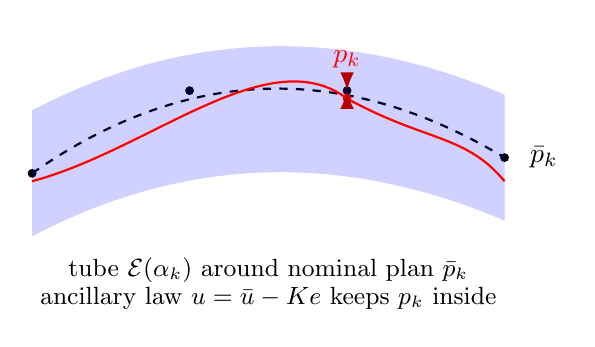
\begin{tikzpicture}[>=Latex,line width=0.8pt]
% nominal trajectory
\draw[dashed] (0,0) .. controls (2,1.4) and (4,1.4) .. (6,0.2);
\foreach \x/\y in {0/0, 2/1.05, 4/1.05, 6/0.2} {\fill (\x,\y) circle (1.6pt);}
\node at (6.5,0.2) {$\bp_k$};
% tube
\begin{scope}[opacity=0.18]
\fill[blue] (0,0) .. controls (2,1.4) and (4,1.4) .. (6,0.2)
  -- (6,-0.6) .. controls (4,0.25) and (2,0.25) .. (0,-0.8) -- cycle;
\fill[blue] (0,0) .. controls (2,1.4) and (4,1.4) .. (6,0.2)
  -- (6,1.0) .. controls (4,1.85) and (2,1.85) .. (0,0.8) -- cycle;
\end{scope}
% true state
\draw[red,thick] (0,-0.1) .. controls (1.5,0.3) and (3,1.7) .. (4,0.95)
  .. controls (5,0.4) and (5.5,0.5) .. (6,-0.1);
\fill[red] (4,0.95) circle (1.6pt);
\node[red] at (4,1.45) {$p_k$};
\draw[<->,red!70!black] (4,1.05) -- (4,1.05);
\node[align=center] at (3,-1.4) {\small tube $\mathcal{E}(\alpha_k)$ around nominal plan $\bp_k$\\[-2pt]
\small ancillary law $u=\bu-Ke$ keeps $p_k$ inside};
\end{tikzpicture}
\caption{Tube MPC concept. The nominal plan $\bp_k$ (dashed, single-integrator \cref{eq:cumsum}) is
surrounded by the ellipsoidal tube $\mathcal{E}(\alpha_k)$ \cref{eq:ellipsoid}. The ancillary law
\cref{eq:ancillary} regulates the true state $p_k$ (red) toward $\bp_k$; the tube radius $\alpha_k$ adapts to
the EKF covariance \cref{eq:alpha}.}
\label{fig:tube}
\end{figure}

% =====================================================================
\section{Event-triggered Tube MPC}
\label{sec:eventtrigger}

Standard Tube MPC re-solves the nominal problem every step. To respect a $150$\,ms control budget, the
ancillary node runs at $20$\,Hz but requests a \emph{replan} only when one of four prioritised conditions
fires (\code{uav\_ancillary\_node.py}). Let $t$ be the current time and let $\tau_\ell$ be the last fire time
of level $\ell$.

\paragraph{Level 1a --- Tube exit (critical, no lockout).} The set-membership test on the ellipsoid
\cref{eq:ellipsoid}:
\begin{equation}
\text{fire}\quad\Longleftrightarrow\quad e_k^\top P_0\,e_k \;>\; \alpha_k^2 .
\label{eq:trig1a}
\end{equation}
This is the literal robustness trigger: the true state has left the tube, so the current plan is no longer
guaranteed to contain it. It fires immediately, with no lockout.

\paragraph{Level 1b --- ArUco covariance spike ($1$\,s lockout).} A sudden estimation-quality collapse:
\begin{equation}
\text{fire}\quad\Longleftrightarrow\quad
\tr\Sigma_{xy}(t) > 0.12 \ \ \wedge\ \ \tr\Sigma_{xy}(t) > 1.5\cdot\tr\Sigma_{xy}(t-\delta),\ \ \delta\approx0.5\text{ s},
\label{eq:trig1b}
\end{equation}
and $t-\tau_{1b}>1$\,s.

\paragraph{Level 2 --- Curvature anticipation ($1$\,s lockout).} Over the first two segments of the UGV
predicted path, estimate the discrete curvature
\begin{equation}
\kappa_i = \frac{|\Delta\theta_i|}{\Delta s_i + 10^{-6}},\qquad
\Delta\theta_i = \mathrm{wrap}(\theta_{i+1}-\theta_i),\ \ \Delta s_i=\norm{p_{i+1}-p_i},
\label{eq:curv}
\end{equation}
and fire iff $\max_i\kappa_i > 0.4$ (and $t-\tau_2>1$\,s). This anticipates a turn so the UAV can climb to
widen the footprint before the UGV reaches it.

\paragraph{Level 3 --- Drift maintenance ($1$\,s lockout).} A slow-drift safety net:
\begin{equation}
\text{fire}\quad\Longleftrightarrow\quad \tr\Sigma_{xy}(t)>0.07 \ \ \wedge\ \ (t-t_{\text{replan}})>T_{\min},
\quad T_{\min}=3\text{ s}.
\label{eq:trig3}
\end{equation}

\paragraph{Chattering avoidance and feasibility.} Levels 1b/2/3 each carry a $1$\,s lockout, the
implementation's chattering guard (a time-dwell rather than a consecutive-violation counter). A
\emph{bootstrap} trigger requests the first plan, and a TAKEOFF$\to$TRACKING state machine first climbs to
$5$\,m at $0.5$\,m/s.

\paragraph{Why event-triggering preserves robust invariance.} Between triggers the ancillary law
\cref{eq:ancillary} is always active, so the error obeys \cref{eq:errordyn} with $A_K$ Schur; hence
$e_k\in\mathcal{E}(\alpha_k)$ is positively invariant for as long as the plan and radius are held fixed. The
critical trigger \cref{eq:trig1a} fires \emph{exactly} when invariance would be lost, forcing a fresh plan
recentred on the current state; under the standard recursive-feasibility argument
(\cref{sec:validation}) this restores a feasible nominal trajectory. Triggers 1b/2/3 are \emph{anticipatory}
(they replan before the tube is violated), so they can only improve feasibility margins; their lockouts
prevent solve storms without affecting the critical guarantee, which has no lockout. The argument is the
standard one for event-triggered Tube MPC and relies on the tube being a true RPI set --- an assumption
inherited from the (absent) RPI design, see \cref{sec:impl}.

% =====================================================================
\section{Extended Kalman Filter with view-quality coupling}
\label{sec:ekf}

The EKF (\code{ekf\_node.py}) estimates the UGV belief $(\mu,\Sigma)$ over the $5$-state
$x_{\text{ugv}}=[x,y,\theta,v,\omega]^\top$ at a $20$\,Hz prediction rate ($\Delta t=0.05$\,s), correcting
asynchronously from two sources: wheel odometry and the ArUco pose recovered from the drone image.

\subsection{Prediction}
With process model $f$ \cref{eq:lag,eq:ugv_disc} and the last command,
\begin{align}
\mu^- &= f(\mu,\,u_{\text{ugv}};\Delta t), &
\Sigma^- &= F\,\Sigma\,F^\top + Q,
\label{eq:ekfpredict}
\end{align}
with $Q=\diag(10^{-4},10^{-4},4{\times}10^{-4},10^{-4},2.5{\times}10^{-3})$.

\subsection{Process Jacobian}
The code uses the \emph{first-order (Euler) Jacobian}
\begin{equation}
F = I_5 +
\begin{bmatrix}
0 & 0 & -v\sin\theta\,\Delta t & \cos\theta\,\Delta t & 0\\
0 & 0 &  v\cos\theta\,\Delta t & \sin\theta\,\Delta t & 0\\
0 & 0 & 0 & 0 & \Delta t\\
0 & 0 & 0 & -\alpha_v\,\Delta t & 0\\
0 & 0 & 0 & 0 & -\alpha_\omega\,\Delta t
\end{bmatrix}.
\label{eq:F}
\end{equation}
The bottom two rows are the exact linearisation of the actuator lag \cref{eq:lag} ($\partial v_{k+1}/\partial
v_k=1-\alpha_v\Delta t$, etc.). The top rows are the Jacobian of the \emph{Euler} pose update
$x_{k+1}=x_k+v\cos\theta\,\Delta t$, \emph{not} of the exact arc model \cref{eq:ugv_disc} actually used to
propagate the mean: \cref{eq:F} drops $\partial x/\partial\omega$ and the trapezoidal-mean/lag factors in the
$v$ and $\theta$ partials. For small $\Delta t$ the two Jacobians agree to first order; the mismatch is a
deliberate approximation, recorded in \cref{sec:impl}.

\subsection{Update (Joseph form)}
For a measurement $z=h(x)+\nu$, $\nu\sim\mathcal N(0,R)$, with $H=\partial h/\partial x$,
\begin{align}
S &= H\Sigma^- H^\top + R, & K_{\text{KF}} &= \Sigma^- H^\top S^{-1}, &
\mu^+ &= \mu^- + K_{\text{KF}}\,(z - H\mu^-),
\label{eq:ekfgain}
\end{align}
(with heading innovation wrapped to $(-\pi,\pi]$), and the Joseph-form covariance update for numerical
stability,
\begin{equation}
\boxed{\;\Sigma^+ = (I-K_{\text{KF}}H)\,\Sigma^-\,(I-K_{\text{KF}}H)^\top + K_{\text{KF}}\,R\,K_{\text{KF}}^\top\;}
\label{eq:joseph}
\end{equation}
followed by symmetrisation $\Sigma^+\leftarrow\tfrac12(\Sigma^++\Sigma^{+\top})$. \Cref{eq:joseph} keeps
$\Sigma^+\succeq0$ even under marginal numerics \citep{thrun2005probabilistic}.

\paragraph{Measurement models.} Both are linear, so $H$ is constant.
\begin{itemize}
\item \textbf{Odometry} measures the body velocities, $z=[v,\omega]^\top$, with
\[
H_{\text{odom}}=\begin{bmatrix}0&0&0&1&0\\0&0&0&0&1\end{bmatrix},\qquad
R_{\text{odom}}=\diag(4{\times}10^{-4},\,2.5{\times}10^{-3}).
\]
\item \textbf{ArUco} provides only pose $(x,y,\theta)$. The code forms a \emph{full-state pseudo-measurement}
by padding with the current velocity estimate, $z=[x,y,\theta,\mu_v,\mu_\omega]^\top$, and uses $H=I_5$. The
last two rows carry no new information (their innovation is zero by construction) and contribute only through
$R$ --- a modelling artefact noted in \cref{sec:impl}, not a true $5$-dimensional observation.
\end{itemize}

\subsection{View-quality-coupled measurement noise}
\emph{Intuition.} When the drone is far from optimal --- target near the edge of the footprint or altitude far
from $z_\opt$ --- the ArUco pose is unreliable and should be trusted less. The code therefore scales the ArUco
noise \emph{inversely} with the geometric view-quality score $q_k\in(0,1]$ (\cref{sec:viewquality}):
\begin{equation}
\boxed{\;R_k = \frac{R_{\text{full}}}{q_k + 10^{-3}}\;}
\label{eq:Rk}
\end{equation}
with $R_{\text{full}}=\diag(2.5{\times}10^{-3},2.5{\times}10^{-3},10^{-2},4{\times}10^{-4},2.5{\times}10^{-3})$.
As $q_k\to1$ (excellent view) $R_k\to R_{\text{full}}$; as $q_k\to0$ (poor view) $R_k\to\infty$ and the
update \cref{eq:ekfgain} ignores the ArUco measurement. This is the second arm of the perception--control
coupling: the UAV's geometry, via $q_k$, modulates how much the ground estimate trusts its own perception.

\begin{quote}\small
\textbf{Note on form.} An alternative pixel-based model $R_k=R_{\text{base}}(1+\alpha\norm{d_{\text{pixel}}}^2)$
(noise growing with the marker's pixel distance from frame centre) is a common heuristic, but it is \emph{not}
what the code implements. The implementation uses the inverse-view-quality form \cref{eq:Rk}, where $q_k$ is a
function of the $3$-D UAV/UGV geometry, not pixel coordinates.
\end{quote}

% =====================================================================
\section{Belief-space MPC for the UGV}
\label{sec:beliefmpc}

The ground controller (\code{belief\_mpc\_node.py}) is an information-aware NMPC: it tracks the lane while
actively keeping itself observable. Following belief-space planning \citep{platt2010belief,vandenberg2012motion}
the planning state is augmented with the covariance,
\begin{equation}
\xi_k = (\mu_k,\Sigma_k),
\end{equation}
and the controller propagates \emph{both} the mean (via $f$, \cref{eq:ugv_disc}) and the covariance through
the horizon, so that it can reason about how its own motion will change the quality of the drone's estimate.

\subsection{Covariance propagation with FoV gating}
At each predicted step the controller forms the no-observation prediction $\Sigma_{\text{pred}}=F\Sigma F^\top
+Q$ and a post-measurement covariance $\Sigma_{\text{obs}}$ from a Joseph update \cref{eq:joseph} with the same
dynamic noise \cref{eq:Rk}. Whether a measurement is available depends \emph{smoothly} on visibility through
the sigmoid gate
\begin{equation}
\gamma = \frac{1}{1+\exp\!\big(\beta\,(d-r_{\fov})\big)},\qquad \beta=5,
\label{eq:gate}
\end{equation}
($\gamma\to1$ inside the footprint $d<r_{\fov}$, $\gamma\to0$ outside), and the predicted covariance is the
blend
\begin{equation}
\boxed{\;\Sigma_k = (1-\gamma)\,\Sigma_{\text{pred}} + \gamma\,\Sigma_{\text{obs}}\;}
\label{eq:blend}
\end{equation}
This is the predictive heart of the method: the MPC simulates the future estimator and optimises against it.

\subsection{Cost function (as implemented)}
With horizon $N=5$, $\Delta t=0.2$, mean $\mu_k$, target $x^{\text{ref}}=p_{\text{tgt}}$, heading error
$e_{\theta,k}$, control increment $\Delta u_k=u_k-u_{k-1}$, and weights $w_d=10,\ w_h=10,\ w_r=5,\ \lambda=1,\
w_{\fov}=2$,
\begin{equation}
\boxed{\;
J_{\text{ugv}} = \sum_{k=0}^{N-1}\Big[\,
w_d\,\norm{p_k-p_{\text{tgt}}}^2
+ w_h\,e_{\theta,k}^2
+ w_r\,\norm{\Delta u_k}^2
+ \lambda\,\tr\Sigma_k
+ w_{\fov}\,c_{\fov}(x_k)\,\Big]\;}
\label{eq:ugvcost}
\end{equation}
The FoV-exit penalty is a \textbf{one-sided quadratic hinge} (a ReLU$^2$ soft constraint --- not a log- or
inverse-barrier):
\begin{equation}
c_{\fov}(x_k) = \big(\max(0,\,d_k-r_{\fov})\big)^2 .
\label{eq:cfov}
\end{equation}
\textbf{Per-term rationale.} (i) $w_d$: track the lane-centreline waypoint. (ii) $w_h$: align heading toward
the target --- switched off near the target (when squared distance $<0.05$\,m$^2$, i.e.\ within $\approx0.22$\,m)
to avoid spin-in-place. (iii) $w_r$: penalise control increments for smoothness. (iv) $\lambda\tr\Sigma_k$:
the information term --- prefer manoeuvres the drone can estimate well (lowers predicted uncertainty).
(v) $w_{\fov}c_{\fov}$: directly discourage leaving the footprint \cref{eq:fovconstraint}. Terms (iv)--(v)
are what make the controller ``belief-coupled'' and are absent from ECC and from the baseline controllers
(\code{mpc\_node}: only (i)--(iii) with $w_h=2$).

\subsection{Resulting NLP.} The problem
\[
\min_{\{u_0,\dots,u_{N-1}\}} J_{\text{ugv}}
\quad\text{s.t.}\quad \text{\cref{eq:ugv_disc,eq:blend}},\ \ 0\le v\le0.22,\ |\omega|\le2,
\]
is a nonlinear program (the covariance rollout makes it non-convex) solved by SLSQP
\citep{nocedal2006numerical} with \code{maxiter}=20; the first control is applied and the full rollout is
published as the reference goal $g$ for the UAV planner of \cref{sec:tube}.

% =====================================================================
\section{View-quality metric and altitude adaptation}
\label{sec:viewquality}

The scalar that couples geometry to both the EKF (\cref{eq:Rk}) and the belief MPC gate (\cref{eq:gate}) is the
differentiable view-quality score $q$ (\code{view\_quality.py}). It is the \emph{product of three} factors:
\begin{equation}
\boxed{\;
q(d,z) =
\underbrace{\frac{1}{1+\exp\!\big(\beta(d-r_{\fov})\big)}}_{\text{(a) FoV-boundary gate}}
\cdot
\underbrace{\exp\!\Big(-\frac{d^2}{2\sigma_{xy}^2}\Big)}_{\text{(b) centering}}
\cdot
\underbrace{\exp\!\Big(-\frac{(z-z_\opt)^2}{2\sigma_z^2}\Big)}_{\text{(c) altitude precision}}\;}
\label{eq:q}
\end{equation}
with $r_{\fov}=z\tan(\fov/2)$ \cref{eq:rfov} (clamped $\ge0.1$), $d$ the horizontal UAV$\to$UGV distance,
$\sigma_{xy}=r_{\fov}/2$, $\beta=5$, $z_\opt=5$\,m, $\sigma_z=3$\,m.

\paragraph{Factor (a)} is a smooth gate going $1\to0$ as the target crosses the footprint radius $r_{\fov}$
(at $d=r_{\fov}$, value $\tfrac12$); $\beta$ sets the roll-off sharpness. \textbf{Factor (b)} rewards keeping
the target near the optical axis, with spread tied to the footprint ($\sigma_{xy}=r_{\fov}/2$). \textbf{Factor
(c)} is a Gaussian preferring the precision-optimal altitude $z_\opt$: too low loses footprint, too high loses
pixel resolution. Here $\sigma_z$ \emph{is} a genuine standard deviation (contrast the planner weight $w_z$ of
\cref{eq:uavcost}, which shares the code name \code{sigma\_z} but is a plain quadratic weight). The product is
differentiable, hence safe inside the gradient-based SLSQP solvers; a central-difference gradient helper is
also provided.

\paragraph{Altitude adaptation.} There is no separate altitude controller. Altitude emerges from the planner
cost \cref{eq:uavcost}: factor (c)'s preference enters as the $w_z(z-z_\opt)^2$ term, while the visibility
term $w_{\text{alt}}\norm{\bp^{xy}-g^{xy}}^2/(z^2+0.1)$ rewards climbing when the target is laterally
offset (a higher $z$ enlarges $r_{\fov}$ and shrinks the penalty). The curvature trigger \cref{eq:curv} causes
a replan before a turn, and the resolved plan then chooses to climb if doing so lowers \cref{eq:uavcost}.
Thus ``climb into turns to widen the field of view'' is an \emph{emergent} optimum, not a hand-coded rule.

\paragraph{Perception scale caveat.} The pixel$\to$metre conversion used to recover the ArUco world position,
$s = 2h\tan(\fov/2)/W$ (image width $W$), is computed \emph{once} with a hard-coded $h=5$\,m. Because altitude
is in fact a decision variable, the metric scale --- and the $x,y$ fed to the EKF --- are correct only at
$z=5$ and are off by a factor $z/5$ otherwise (\cref{sec:impl}).

% =====================================================================
\section{Validation: stability, recursive feasibility, and ISS}
\label{sec:validation}

We are explicit about what is proven, what is inherited from cited theorems under assumptions, and what is
only empirical.

\paragraph{Recursive feasibility of Tube MPC.} Under (A1) and assuming $\Omega$ is a true RPI set for
\cref{eq:errordyn} with tightened constraints \cref{eq:tighten}, the nominal problem is recursively feasible:
a feasible plan at step $k$ yields a feasible candidate at $k{+}1$ by shifting and appending a terminal step,
and the true state remains in $\bar\Xset\oplus\Omega\subseteq\Xset$
\citep[Thm.~1]{mayne2005robust}\citep{rakovic2005invariant}. \emph{Caveat:} this guarantee requires the tube
to be a correctly computed RPI set. The implementation uses the loaded/fallback ellipsoid \cref{eq:ellipsoid}
with gains not derived here, and does not implement constraint tightening; so recursive feasibility holds
\emph{for the idealized design} and is assumed, not verified, for the code.

\paragraph{Input-to-state stability (ISS).} For \cref{eq:errordyn} with $A_K$ Schur and $w_k\in\W$ bounded,
the error is ISS: there exist a $\mathcal{KL}$ function $\beta_{\mathrm{ISS}}$ and a $\mathcal K$ function
$\gamma_{\mathrm{ISS}}$ with $\norm{e_k}\le\beta_{\mathrm{ISS}}(\norm{e_0},k)+\gamma_{\mathrm{ISS}}(\sup_i
\norm{w_i})$, and the true state converges to the tube $\Omega$ around the nominal trajectory
\citep{mayne2005robust}. For the implemented $A_K=0.6\,I_3$ this is immediate (a contraction with disturbance),
giving $\norm{e_{k+1}}\le0.6\norm{e_k}+\sup\norm{w}$, hence $\limsup_k\norm{e_k}\le\sup\norm{w}/0.4$. The
nominal MPC's own stability is the standard result of \cref{sec:mpc}
\citep{mayne2000constrained,rawlings2017model}.

\paragraph{Belief-MPC stability.} Adding $\lambda\tr\Sigma_k$ and $c_{\fov}$ to the stage cost
\cref{eq:ugvcost} does \emph{not} automatically preserve nominal-MPC stability guarantees: the covariance
rollout \cref{eq:blend} makes the cost non-convex and state-dependent in a way the standard terminal-cost
machinery does not cover. We rely on \cref{eq:ugvcost} being a valid Lyapunov candidate under mild assumptions
(bounded covariance, persistent observability) in the spirit of belief-space planning
\citep{platt2010belief,vandenberg2012motion}; \textbf{we have not proven this formally}, and the controller
runs with no terminal set or terminal cost.

\paragraph{Numerical validation.} The package's README reports a comparison table (mean tracking error
$1.037\to0.463$\,m, $-55.3\%$; ArUco visibility $46.3\%\to87.0\%$) attributing the gains to the belief
coupling and adaptive tube. These figures are \emph{empirical and external}: the code report (\code{report.html})
notes they originate from upstream ``Phase\,1/Phase\,3'' artifacts not contained in this package and could not
be reproduced from these sources alone. We therefore cite them as indicative empirical evidence, \textbf{not}
as formal proof, and recommend re-running the logger (\code{experiment\_logger.py}) to regenerate them before
relying on the numbers.

% =====================================================================
\section{Implementation notes: theory vs.\ code}
\label{sec:impl}

This section lists, honestly, where the implementation deviates from the idealized derivations above.

\begin{enumerate}
\item \textbf{UAV model.} Theory of robust MPC is usually posed on a double integrator with acceleration
input; the code uses the \emph{single integrator} \cref{eq:uav_disc} with velocity input ($A_d=I_3$,
$B_d=\Delta t\,I_3$). All derivations here use the implemented form.

\item \textbf{Tube gains $K,P_0$.} Not computed (no LQR/Riccati, no mRPI iteration \cref{eq:mrpi}). Loaded from
\code{tube\_params.npz}; absent that file, fallback $K=2I_3$, $P_0=6.86\,I_3$. The Schur and Lyapunov
properties assumed in \cref{sec:tube,sec:validation} hold for the fallback but the designed RPI set is
external (``Phase 1'').

\item \textbf{Constraint tightening} \cref{eq:tighten} is not implemented; there are no explicit
$\Xset,\Uset,\Omega$ in the code. The tube is the ellipsoid \cref{eq:ellipsoid} with adaptive radius
\cref{eq:alpha}.

\item \textbf{Nominal/ancillary timestep mismatch.} The planner emits the plan at $\Delta t=0.2$\,s, but the
ancillary interpolator \code{get\_nominal\_state} assumes $0.3$\,s steps. The interpolated $\bp$ and the
finite-difference $\bu$ are therefore time-distorted --- a likely bug; the tracker follows a stretched version
of the plan.

\item \textbf{EKF Jacobian.} \Cref{eq:F} is the Euler Jacobian, not the exact derivative of the arc model
\cref{eq:ugv_disc} used for the mean. First-order accurate in $\Delta t$.

\item \textbf{ArUco pseudo-measurement.} $H=I_5$ with $z$'s velocity entries set to the current estimate; the
$v,\omega$ rows carry no information (\cref{sec:ekf}).

\item \textbf{Altitude limits.} $z_{\min}=3,z_{\max}=10$ are declared but never enforced as constraints; only
the velocity bound $v_z\in[-1,1]$ and the soft $z_\opt$ cost shape altitude.

\item \textbf{Inconsistent $z_\opt$.} Planner default $5.0$, launch file passes $6.0$, \code{view\_quality.py}
hard-codes $5.0$; the planner and the metric driving the EKF can disagree on the ``optimal'' altitude.

\item \textbf{Perception scale.} Pixel$\to$metre scale fixes $h=5$\,m once (\cref{sec:viewquality}); incorrect
by $z/5$ whenever the planned altitude $z\ne5$.

\item \textbf{Solver settings.} SLSQP with \code{ftol}$=10^{-3}$; \code{maxiter}$=15$ (UAV planner),
$20$ (UGV MPCs). Horizons $N=10$ (UAV, $\Delta t=0.2$), $N=5$ (UGV, $\Delta t=0.2$); EKF predict
$\Delta t=0.05$ ($20$\,Hz); ancillary loop $20$\,Hz.

\item \textbf{Trigger form.} The tube-exit trigger is the ellipsoidal test \cref{eq:trig1a}, not a polytopic
$\max(\Omega_H e-\Omega_h)>0$; chattering is handled by $1$\,s time-lockouts on levels 1b/2/3, not by an
$n_{\text{thresh}}$ consecutive-violation counter.
\end{enumerate}

% =====================================================================
\bibliographystyle{plainnat}
\bibliography{theory_report}

\end{document}
